La gente de Bridgetown quería construir un puente que cruzara un río cercano.
Como eran muy malos nadadores, su maestro Trigonomos aceptó medir el ancho del río sin cruzarlo.
Trigonomos vió un árbol al otro lado del río y marcó el punto que estaba directamente frente a él.
Después caminó hasta otro punto que estaba 10 metros río abajo y encontró que el ángulo formado
por su lado del río y la línea que lo conectaba con el árbol era 40$^\circ$.\\
\begin{figure}[H]
    \begin{center}
        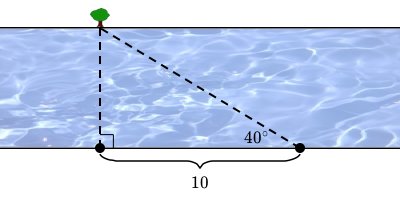
\includegraphics[width=0.5\textwidth]{../images/river1.png}
    \end{center}
    \caption{Imagen satelital del rio en Bridgetown.}
    \label{fig:river1}
\end{figure}
\textbf{¿Cuál es el ancho el río?}\\
\textit{Redondea tu respuesta final a la centésima más cercana.}